\section{核心转向：把记忆从一维文本搬到二维画布}

本章的结论是：MemOCR 的第一层创新是表示空间转向。传统文本记忆把历史压缩成线性状态，MemOCR 先在 text domain 起草带有版面意图的 para-textual memory，再通过 renderer 转成 visual memory，让模型在 vision domain 读取带有显著性、层级和密度差异的记忆画布。

\begin{importantbox}{本章核心判断}
二维画布的价值在于把“内容”和“优先级”一起写进记忆。文本摘要主要回答内容是什么；视觉记忆还能表达内容应放在显著标题区、普通正文区、辅助细节区，进而影响压缩后哪些证据更容易被模型读到。
\end{importantbox}

\subsection{传统文本记忆如何迭代更新}

在转向 MemOCR 之前，讲者先展示了两类文本记忆基线。第一类以 MemAgent 为代表：模型把长上下文切成若干片段，文本记忆智能体逐段处理。处理第一个片段后，它形成一个 memory state；处理第二个片段时，它带着前一个 memory state 继续更新；如此迭代，直到所有原始上下文片段都被消化，最终记忆再交给回答模型。

第二类以 Mem-$\alpha$ 一类工作为代表：系统拆出独立的 memory agent 和 answer agent。memory agent 专门遍历或管理记忆库，抽取与问题相关的信息；更大的 large language model 再利用这些信息回答问题。这个结构比单一摘要更灵活，因为记忆管理和问题回答可以分工。

\begin{figure}[H]
\centering
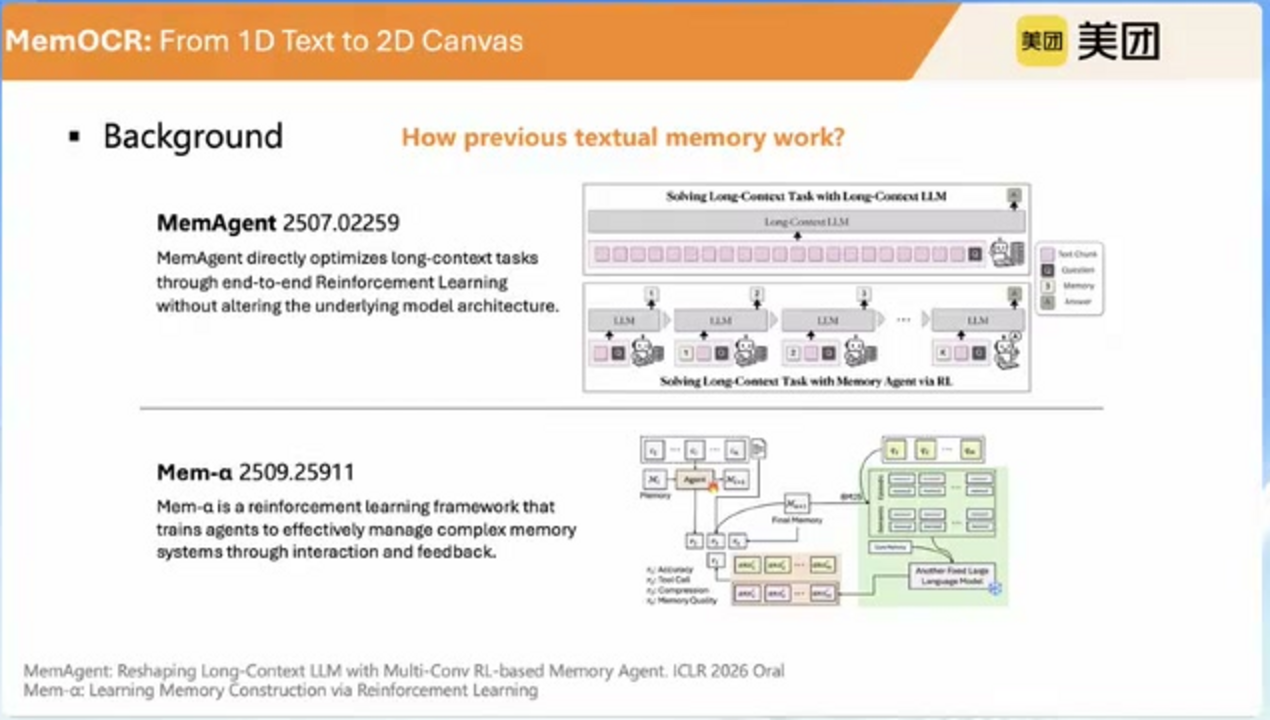
\includegraphics[width=0.82\linewidth,height=0.36\textheight,keepaspectratio]{figures/selected/fig02_textual_memory_baselines.png}
\caption{文本记忆基线的共同结构：历史片段被逐段处理成 memory state，再由回答模型消费最终记忆。\protect\footnotemark}
\label{fig:textual-memory-baselines}
\end{figure}
\footnotetext{视频画面时间区间：00:05:30--00:06:00。}

图~\ref{fig:textual-memory-baselines} 中的共同点值得抓住：无论是逐段更新，还是 memory agent 与 answer agent 分工，最终记忆仍主要以文本形式存在。文本状态便于生成和拼接，却难以表达“这条信息更应该抗压缩，那条信息可以被弱化”。

\subsection{从 text domain 到 vision domain}

MemOCR 提出的范式转移是从 \textit{text domain} 进入 \textit{vision domain}。这一转向包含两个阶段。第一阶段是 \textit{memory drafting}：模型在文本域浏览检索到的文章、上下文窗口或历史片段，并反复更新一份带有布局意图的 \textit{para-textual memory}。第二阶段是 \textit{memory reading}：这份副文本记忆经过 renderer 渲染为图像，形成最终被视觉语言模型读取的 \textit{visual memory}。

为帮助理解，可以把历史片段集合写成：

$$
H = \{h_1, h_2, \ldots, h_n\}
$$

传统文本记忆把这些片段压缩成一段线性状态：

$$
M_{\text{text}} = f_{\theta}(H)
$$

MemOCR 则先生成带有版面意图的副文本记忆，再把它映射到视觉画布：

$$
V = R(M_{\text{para}})
$$

这里的符号含义如下：

\begin{itemize}
  \item $H$：历史交互或检索到的上下文片段集合。
  \item $h_i$：第 $i$ 个历史片段。
  \item $M_{\text{text}}$：线性文本记忆状态。
  \item $f_{\theta}$：把历史片段压缩为文本记忆的模型或策略。
  \item $M_{\text{para}}$：带有版面意图的副文本记忆。
  \item $R$：renderer，把副文本记忆渲染成图像。
  \item $V$：最终由视觉模型读取的视觉记忆。
\end{itemize}

这些公式是讲义为解释机制建立的抽象，用来表达信息形态的变化。它们的作用类似地图：让读者看到从历史片段到文本记忆、再到视觉记忆的路径。

\subsection{渲染器的角色：把记忆变成可读画布}

renderer 是 MemOCR 中很关键的接口。它把 para-textual memory 渲染成 visual memory，使原本线性的内容获得版面结构。讲者用 Markdown 渲染为 PDF、HTML 渲染为网页作类比：同一段文字经过排版后，会产生标题、段落、强调、列表、区域和空间距离。读者看到 PDF 或网页时，已经能从布局中判断哪部分是主题、哪部分是说明、哪部分是辅助材料。

\begin{figure}[H]
\centering
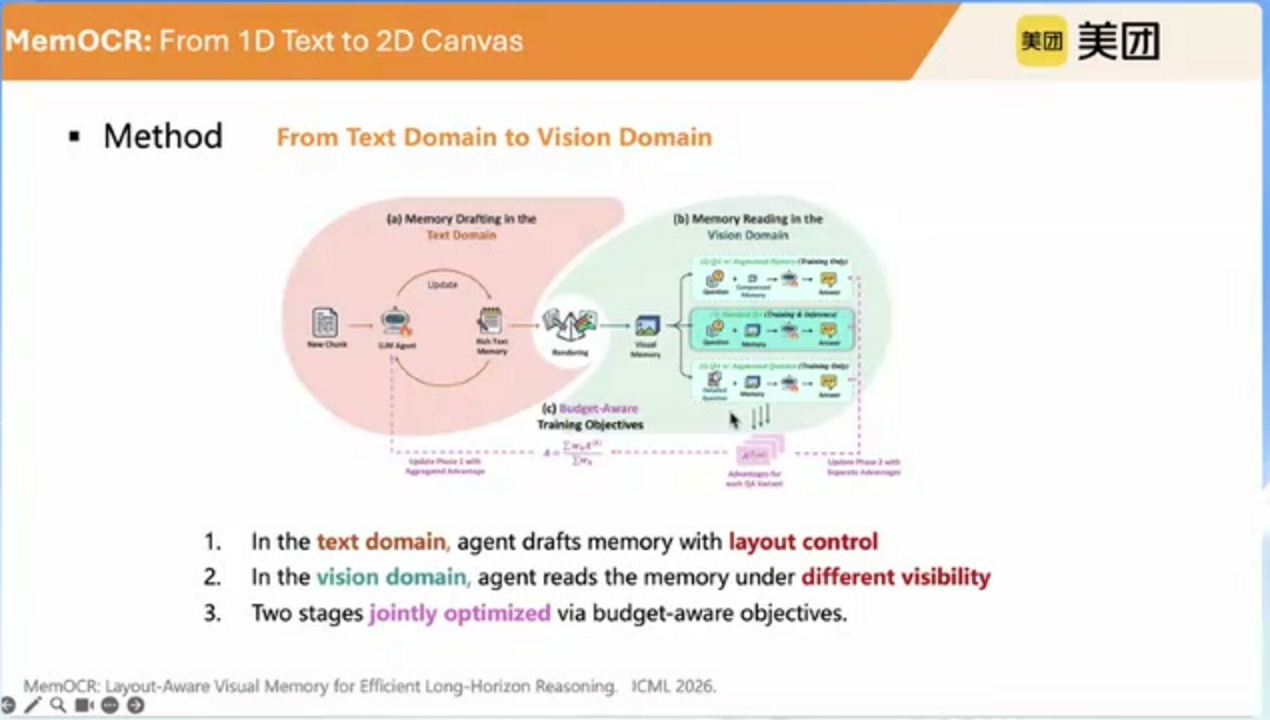
\includegraphics[width=0.86\linewidth,height=0.40\textheight,keepaspectratio]{figures/selected/fig03_text_to_vision_domain.png}
\caption{MemOCR 的 text-to-vision 流程：在 text domain 起草带 layout control 的记忆，在 vision domain 以不同 visibility 读取，并通过 budget-aware objectives 联合优化。\protect\footnotemark}
\label{fig:text-to-vision-domain}
\end{figure}
\footnotetext{视频画面时间区间：00:07:00--00:07:30。}

图~\ref{fig:text-to-vision-domain} 给出了这个流程的全貌。左侧是文本域的 memory drafting：新片段进入后，LLM agent 更新 rich text memory。中间的 rendering 把富文本记忆转为 visual memory。右侧是视觉域的 memory reading：模型在标准 QA、压缩记忆 QA、细节问题 QA 等不同训练条件下读取同一类视觉记忆。

\begin{knowledgebox}{para-textual memory 的直觉}
\textit{Para-textual memory} 可以理解为“即将被排版的记忆草稿”。它依然由文本构成，却已经包含版面意图，例如标题层级、加粗、分区、列表和信息密度安排。它像一份 Markdown 草稿：源文件看起来是文本，渲染后会成为带层级结构的页面。
\end{knowledgebox}

这里的核心机制是 \textit{layout control}。它让模型通过版面控制信息的可见性和显著性：关键证据可以进入标题、加粗块或更醒目的区域；supporting facts 可以放在正文或辅助区域；细节可使用更高密度的写法承载。若后续 image token 预算降低，模型仍更可能读取到醒目区域的内容。

\begin{warningbox}{表示转向带来的新风险}
视觉记忆引入了读取能力约束。画布能表达优先级，也会受到下采样、OCR 能力、字体大小和视觉语言模型识别能力限制。若信息写得过密，visual memory 会从“可压缩的画布”退化成“看不清的截图”。这也是后续失败模式分析必须保留的边界。
\end{warningbox}

\subsection{本章小结}

本章解释了 MemOCR 的核心表示转向。传统文本记忆通过逐段更新或 memory agent 管理历史，但最终仍生成线性记忆状态；MemOCR 则把记忆拆成 text-domain drafting、renderer 渲染和 vision-domain reading 三步。副文本记忆保留内容与版面意图，renderer 把它变成可读画布，visual memory 让模型借助显著性和布局读取不同优先级的信息。下一章的关键问题随之出现：模型怎样学会在不同 memory budget 下可靠读取这种视觉记忆。
